\documentclass[12pt,a4paper]{article}
\usepackage[utf8]{inputenc} %polskie znaki
\usepackage[T1]{fontenc}	%polskie znaki
\usepackage{amsmath}		%matematyczne znaczki :3
\usepackage{enumerate}		%Dodatkowe opcje do funkcji enumerate
\usepackage{geometry} 		%Ustawianie marginesow
\usepackage{graphicx}		%Grafika
\usepackage{wrapfig}		%Grafika obok textu
\usepackage{float}			%Allows H in fugire
\usepackage{hyperref}		%Allows hyperlinks
%\pagestyle{empty} 			%usuwa nr strony
\usepackage{todonotes}		%Todo notatki
\usepackage{lipsum}         %Lorem text
\usepackage{ntheorem}   	% for theorem-like environments
\usepackage{mdframed}   	% for framing
\usepackage{subcaption}		% subfigure (image placing)
\usepackage{pdfcomment}		% Komentarze (z bazowego pdf'a)
\usepackage{xparse}			% New commands with optional arguments
\usepackage{ifthen}			% If then - funkcje!
\usepackage{expl3}			% Deklarowanie zmiennych

\newgeometry{tmargin=2cm, bmargin=2cm, lmargin=2cm, rmargin=2cm} 

%Counter commands{
	\newcounter{counter} % Creates a new counter
	\setcounter{counter}{1} % Sets the counter to 5
	\newcommand{\counter}[1]{
		\arabic{#1} \stepcounter{#1} 
	}
	\newcommand{\counterreset}[1]{\setcounter{#1}{1}}
	%}

%Define styles{
	\theoremstyle{break}
	\theoreminframepreskip{0.5cm}
	\theoremheaderfont{\bfseries}
	\newmdtheoremenv[%
	linecolor=white,%
	innertopmargin=\topskip,
	shadowsize=0,%
	innertopmargin=5,%
	innerbottommargin=5,%
	leftmargin=10,%
	rightmargin=10,%
	backgroundcolor=gray!20,%
	innertopmargin=0pt,%
	ntheorem]{zad}{Zadanie}
	
	\mdfdefinestyle{zadanie}{
		linecolor=white,%
		innertopmargin=5,%
		innerbottommargin=5,%
		leftmargin=10,%
		rightmargin=10,%
		backgroundcolor=gray!20,%
		innertopmargin=8,
		innerbottommargin=8,
		skipabove = 5,
	}
	\mdfdefinestyle{wzor}{
		linecolor=cyan,%
		linewidth=2pt,%
		innertopmargin=8,
		innerbottommargin=8,
		leftmargin=10,%
		rightmargin=10,%
		backgroundcolor = white, 
		fontcolor = black,
		skipabove = 5,
		skipbelow = 5,
	}
	%}

%Zadania templatex%{
	\newcommand{\Wzor}[1]{
		\begin{mdframed}[style=wzor]
			\centering #1
		\end{mdframed}
	}
	\newcommand{\ZadanieTextowe}[1]{
		\begin{mdframed}[style=zadanie]
			\textbf{Zadanie \counter{counter} } \\
			#1
		\end{mdframed}
	}
	\newcommand{\Zadanie}[2]{
		\ZadanieTextowe{#1}
		#2
	}
	\newcommand{\ZadanieABCD}[6]{
		\ZadanieTextowe{#1}
		#2 \\\\
		\begin{tabular}{p{7cm} p{7cm}}
			\textbf{A. }#3&
			\textbf{B. }#4\\\\
			\textbf{C. }#5&
			\textbf{D. }#6\\
		\end{tabular}
	}
	\newcommand{\ZadanieABCDEF}[8]{
		\ZadanieTextowe{#1}
		#2 \\\\
		\begin{tabular}{p{7cm} p{7cm}}
			\textbf{A. }#3&
			\textbf{B. }#4\\\\
			\textbf{C. }#5&
			\textbf{D. }#6\\\\
			\textbf{E. }#7&
			\textbf{F. }#8\\\\
		\end{tabular}
	}
	\newcommand{\Zadanietwoxtwo}[5]{
		\ZadanieTextowe{#1}
		\begin{tabular}{p{7cm} p{7cm}}
			\textbf{a)} #2&
			\textbf{b)} #3\\\\
			\textbf{c)} #4&
			\textbf{d)} #5\\\\
		\end{tabular}
	}
	\newcommand{\Zadanietwoxthree}[7]{
		\ZadanieTextowe{#1}
		\begin{tabular}{p{7cm} p{7cm}}
			\textbf{a)} #2&
			\textbf{b)} #3\\\\
			\textbf{c)} #4&
			\textbf{d)} #5\\\\
			\textbf{e)} #6&
			\textbf{f)} #7\\\\
		\end{tabular}
	}
	\newcommand{\Zadanietwoxfour}[9]{
		\ZadanieTextowe{#1}
		\begin{tabular}{p{7cm} p{7cm}}
			\textbf{a)} #2&
			\textbf{b)} #3\\\\
			\textbf{c)} #4&
			\textbf{d)} #5\\\\
			\textbf{e)} #6&
			\textbf{f)} #7\\\\
			\textbf{g)} #8&
			\textbf{h)} #9\\\\
		\end{tabular}
	}
	%}

\newcommand{\tg}{\text{tg}}
\newcommand{\ctg}{\text{ctg}}
\newcommand{\UkladRownan}[2]{
	$\left\{
	\begin{array}{l}
		#1 \\
		#2
	\end{array}
	\right.$
}

\begin{document}
	\begin{center}
		\LARGE Funkcja kwadratowa
	\end{center}
	
	\Zadanie{Uzupełnij tabelę oraz podaj własności fukcji kwadratowej (zbiór wartości, przedziały monotoniczności, maksimum/minimum, wierzchołek i miejsca zerowe)}{
		\begin{tabular}{| p{5cm}| p{5cm}| p{5cm}|}\hline
			\begin{center}
				Postać kanoniczna
			\end{center}&\begin{center}
			Postać ogólna
		\end{center}&\begin{center}
		Postać iloczynowa
	\end{center}\\
			\hline
			&&\\&$x^2-4x+3$&\\&&\\\hline
			&&\\&&$2(x-1)(x-3)$\\&&\\\hline
			&&\\&$x^2-6x+9$&\\&&\\\hline
			&&\\$-\frac{1}{2}(x-3)^2+9$&&\\&&\\\hline
			&&\\&$-3x^2+6x$&\\&&\\\hline
			&&\\&&$-(x+2)(x-6)$\\&&\\\hline
			&&\\&$x^2+5x+13$&\\&&\\\hline
			&&\\$-2(x+2)^2-2$&&\\&&\\\hline
		\end{tabular}
	}
	\ZadanieTextowe{Dana jest funkcja kwadratowa, która ma tylko jedno miejsce zerowe oraz jest rosnąca w przedziale $\langle -2,\infty )$. Wiedząc, że przechodzi ona przez punkt $P=(0,2)$ wyznacz jej w wzór w postaci ogólnej.}
	\ZadanieTextowe{Pewna funkcja kwadratowa przyjmuje największą wartość równą 3, a jej dwa miejsca zerowe to -2 i 4. Wyznacz jej wzór w postaci ogólnej.}
	\newpage
	\ZadanieTextowe{Rozwiąż równania i nierówności:}
	\begin{enumerate}[a)]
		\item $x^2+2x=3$
		\item $2x^2+6x-8=0$
		\item $-x^2+4x-4=0$
		\item $2x^2-7x=15$
		\item $x^2+4x-5=0$
		\item $x^2+7x+12\leq 0$
		\item $x^2-16>0$
		\item $-x^2+6x-13<0$
		\item $2x^2+8x+8>0$
		\item $x^2-6x+6<0$
		\item $x^2-10x+25\leq0$
		\item $x(2-x)<3x-6$
		\item $\frac{x+2}{3}-x^2<4$
		\item $10(x-5)-2x(x-5)=2$
		\item $4(x+1)^2-(2x-2)^2<16$
	\end{enumerate}

	\newpage
	\counterreset{counter}
	
	\Zadanie{Informacja do zadań \textbf{2-4}.}{
Poniżej przedstawiono fragment funkcji kwadratowej $f(x)$:
\begin{center}
	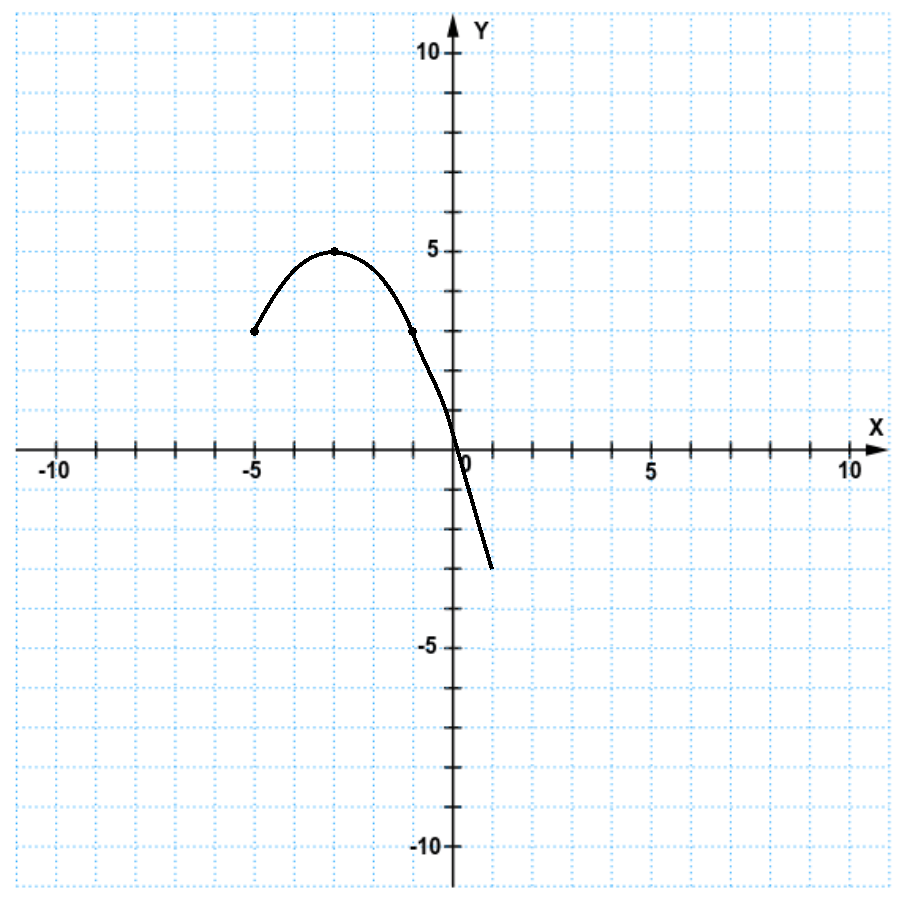
\includegraphics[scale=0.4]{4_1_1.png}
\end{center}	
}
\ZadanieABCD{Dokończ zdanie. Wybierz odpowiedź spośród ABCD}{Oś symetrii tej funkcji kwadratowej da się zapisać za pomocą równania}{$x=3$}{$x=-3$}{$y=5$}{$y=-3$}
	\Zadanie{Zapisz zbiór wartości powyższej funkcji kwadratowej}{
	\vspace{0.5cm}	\dots\dots\dots\dots\dots\dots\dots\dots\dots\dots\dots\dots\dots\dots\dots\dots\dots\dots\dots\dots\dots\dots\dots\dots\dots\dots\dots\dots\dots\dots\dots}
\ZadanieTextowe{Wyznacz wzór tej funkcji kwadratowej w postaci ogólnej.}
\end{document}